\begin{itemize}
\item \textbf{Motivation}
\item in SSP: try all orderings before "no solution"
\item PSP: do not commit to orderings, instantiations, etc.

\item \textbf{Partial Order Plan vs Total Order Plan}
\item POP: "parallel" paths

\item \textbf{PSP}: Backward search from g
\item Each node is \textbf{partial plan}
	\begin{itemize}
	\item \{ part.-instantiated operators (\textbf{steps}) \}
	\item Sets of constraints
	\end{itemize}
\item Refine until solution

\item \textbf{Constraints}
	\begin{itemize}
	\item \textbf{Precedence constraints}: a must precede b
	\item \textbf{Binding constraints}: (in)equality
	\item \textbf{Causal links}: use step a to establish prec p needed by c
	\end{itemize}
\item No more \textbf{flaws} $\rightarrow$ plan

\item \textbf{Representation}
\item P = $\langle$ steps, orderings, bindings, causallinks $\rangle$

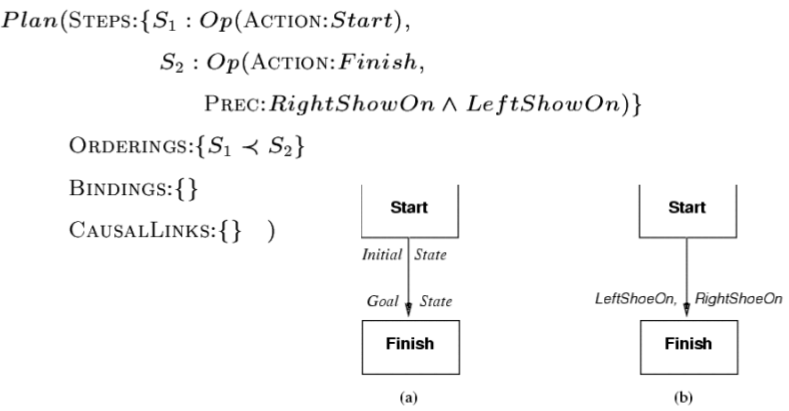
\includegraphics[width=0.48\textwidth]{./img/psp_representation.png}

\end{itemize}